\begin{figure*}[ht]
    \begin{minipage}[t]{0.37\textwidth}
        \centering
        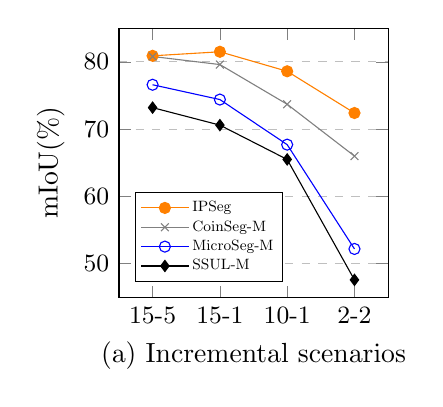
\begin{tikzpicture}
            \begin{axis}[
                xlabel={(a) Incremental scenarios},
                % xlabel={\shortstack{Incremental scenarios \\ \\ (a)}},
                ylabel={mIoU(\%)},
                xmin=0.5, xmax=4.5,
                ymin=45, ymax=85,
                xtick={1,2,3,4},
                xticklabels={\text{\small 15-5},\text{\small 15-1},\text{\small 10-1},\text{\small 2-2}},
                ytick={50, 60, 70, 80},
                yticklabels = {\text{\small 50}, \text{\small 60}, \text{\small 70}, \text{\small 80}},
                legend style={
                    font=\small, 
                    at={(0.05,0.05)}, 
                    anchor=south west,
                    inner sep=2pt, % 内边距
                    outer sep=1pt, % 外边距
                    nodes={scale=0.6, transform shape} % 缩小标志和文字
                },
                ymajorgrids=true,
                grid style=dashed,
                legend cell align={left},
                % width=1\textwidth, % 调整图表的宽度
                width=5cm, % 调整图表的宽度
                height=5cm %0.5\textwidth % 调整图表的高度
            ]
            
            \addplot[
                color=orange,
                mark=*, 
                mark size=2pt % 缩小标记
                ]
                coordinates {
                (1,80.9)(2,81.5)(3,78.6)(4,72.4)
                };
                \addlegendentry{IPSeg}
            
            \addplot[
                color=gray,
                mark=x,
                mark size=2pt % 缩小标记
                ]
                coordinates {
                (1,80.8)(2,79.6)(3,73.7)(4,66.0)
                };
                \addlegendentry{CoinSeg-M}
            
            \addplot[
                color=blue,
                mark=o,
                mark size=2pt % 缩小标记
                ]
                coordinates {
                (1,76.6)(2,74.4)(3,67.7)(4,52.2)
                };
                \addlegendentry{MicroSeg-M}
            
            \addplot[
                color=black,
                mark=diamond*,
                mark size=2pt % 缩小标记
                ]
                coordinates {
                (1,73.2)(2,70.6)(3,65.5)(4,47.6)
                };
                \addlegendentry{SSUL-M}
            
            % \addplot[
            %     color=cyan,
            %     mark=square,
            %     mark size=2pt % 缩小标记
            %     ]
            %     coordinates {
            %     (1,72.4)(2,59.4)(3,34.3)(4,19.4)
            %     };
            %     \addlegendentry{RCIL}
            
            \end{axis}
        \end{tikzpicture}
        % \parbox{0.1cm}{\hfill}
        % \subcaption{}
    \end{minipage}
    \begin{minipage}[t]{0.3\textwidth}
        \centering
        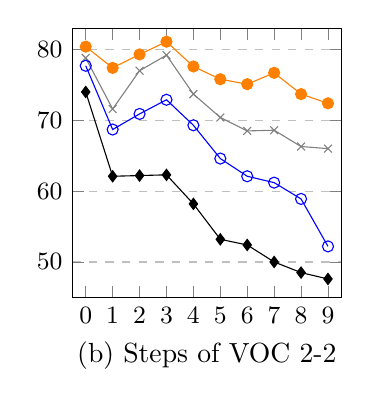
\begin{tikzpicture}
            \begin{axis}[
                xlabel={(b) Steps of VOC 2-2},
                % xlabel={\shortstack{VOC 2-2 \\ \\ (c)}},
                % ylabel={mIoU(\%)},
                xmin=-0.5, xmax=9.5,
                ymin=45, ymax=83,
                xtick={0,1,2,3,4,5,6,7,8,9},
                xticklabels={\text{\small 0}, \text{\small 1}, \text{\small 2}, \text{\small 3}, \text{\small 4}, \text{\small 5}, \text{\small 6}, \text{\small 7}, \text{\small 8}, \text{\small 9}},
                ytick={50, 60, 70, 80},
                yticklabels = {\text{\small 50}, \text{\small 60}, \text{\small 70}, \text{\small 80}},
                legend style={
                    font=\small, 
                    at={(0.05,0.05)}, 
                    anchor=south west,
                    inner sep=2pt,
                    outer sep=1pt,
                    nodes={scale=0.6, transform shape}
                },
                ymajorgrids=true,
                grid style=dashed,
                legend cell align={left},
                % width=1\textwidth,
                width=5cm, % 调整图表的宽度
                height=5cm
            ]
            
            \addplot[
                color=orange,
                mark=*, 
                mark size=2pt
                ]
                coordinates {
                (0,80.4)(1,77.4)(2,79.3)(3,81.1)(4,77.6)(5,75.8)(6,75.1)(7,76.7)(8,73.7)(9,72.4)
                };
                % \addlegendentry{IPSeg}
            
            \addplot[
                color=gray,
                mark=x,
                mark size=2pt
                ]
                coordinates {
                (0,78.8)(1,71.6)(2,77.0)(3,79.2)(4,73.7)(5,70.4)(6,68.5)(7,68.6)(8,66.3)(9,66.0)
                };
                % \addlegendentry{CoinSeg-M}
            
            \addplot[
                color=blue,
                mark=o,
                mark size=2pt
                ]
                coordinates {
                (0,77.7)(1,68.7)(2,70.9)(3,72.9)(4,69.3)(5,64.6)(6,62.1)(7,61.2)(8,58.9)(9,52.2)
                };
                % \addlegendentry{MicroSeg-M}
            
            \addplot[
                color=black,
                mark=diamond*,
                mark size=2pt
                ]
                coordinates {
                (0,74.0)(1,62.1)(2,62.2)(3,62.3)(4,58.2)(5,53.2)(6,52.4)(7,50.0)(8,48.5)(9,47.6)
                };
                % \addlegendentry{SSUL-M}
            
            \end{axis}
        \end{tikzpicture}
        % \subcaption{}
    \end{minipage}
    \begin{minipage}[t]{0.3\textwidth}
        \centering
        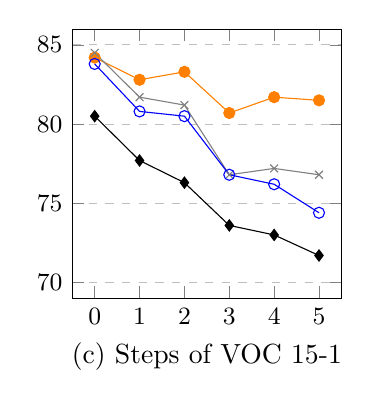
\begin{tikzpicture}
            \begin{axis}[
                xlabel={(c) Steps of VOC 15-1},
                xmin=-0.5, xmax=5.5,
                ymin=69, ymax=86,
                xtick={0,1,2,3,4,5},
                xticklabels={\text{\small 0}, \text{\small 1}, \text{\small 2}, \text{\small 3}, \text{\small 4}, \text{\small 5}},
                % xticklabels={15-5,15-1,10-1,2-2},
                ytick={70,75,80,85},
                yticklabels = {\text{\small 70}, \text{\small 75}, \text{\small 80}, \text{\small 85}},
                legend style={
                    font=\small, 
                    at={(0.05,0.05)}, 
                    anchor=south west,
                    inner sep=2pt,
                    outer sep=1pt,
                    nodes={scale=0.6, transform shape}
                },
                ymajorgrids=true,
                grid style=dashed,
                legend cell align={left},
                % width=1\textwidth,
                width=5cm, % 调整图表的宽度
                height=5cm
            ]
            
            \addplot[
                color=orange,
                mark=*, 
                mark size=2pt
                ]
                coordinates {
                (0,84.2)(1,82.8)(2,83.3)(3,80.7)(4,81.7)(5,81.5)
                };
                % \addlegendentry{IPSeg}
            
            \addplot[
                color=gray,
                mark=x,
                mark size=2pt
                ]
                coordinates {
                (0,84.5)(1,81.7)(2,81.2)(3,76.8)(4,77.2)(5,76.8)
                % (0,0)(1,1)(2,2)(3,3)(4,4)(5,5)
                };
                % \addlegendentry{CoinSeg-M}
            
            \addplot[
                color=blue,
                mark=o,
                mark size=2pt
                ]
                coordinates {
                
                (0,83.8)(1,80.8)(2,80.5)(3,76.8)(4,76.2)(5,74.4)
                };
                % \addlegendentry{MicroSeg-M}
            
            \addplot[
                color=black,
                mark=diamond*,
                mark size=2pt
                ]
                coordinates {
                (0,80.5)(1,77.7)(2,76.3)(3,73.6)(4,73.0)(5,71.7)
                };
                % \addlegendentry{SSUL-M}
            \end{axis}
        \end{tikzpicture}
        % \subcaption{}
    \end{minipage}
    \caption{(a) The overall performance of different methods on Pascal VOC 2012 under 4 scenarios, (b) mIoU visualization on Pascal VOC 2012 2-2, (c) mIoU visualization on Pascal VOC 2012 15-1.}
    \label{fig:performance_voc}
    \vspace{-5pt}
\end{figure*}